%\marginpar{\scriptsize \textcolor{blue}{Michael, take all of these numbers with a grain of salt; we have some regressions and churn in the code, which we hope to wrap up soon and get more stable numbers.}}

\section{Evaluation}
\label{sec:dcache:eval}

This section evaluates our directory cache optimizations,
and seeks to answer the following questions:
\begin{compactenum}
\item How much does each optimization---the lookup fastpath, whole directory caching, and more aggressive negative dentries---improve application performance?  
\item How difficult are the changes to adopt, especially for individual file systems?
%\item Do the changes maintain compatibility with current Linux applications and security modules?
%Does our {\em fastpath} significantly improve directory cache lookup at a cache hit and cause acceptable slow-down at a cache miss?
%\item How much does our solution reduce the synchronization cost for directory cache lookup, and improve multi-core performance and fairness of file system?
%\item How is performance of file systems affected by improving the hit rate at {\tt readdir}, renaming and deletion?
\end{compactenum}


The evaluation includes both 
%{\bf nano-benchmarks} to show impact of our optimization on various directory cache operations,
micro-benchmarks to measure the latency of file system related system calls in best-case and worst-case scenarios,
and a selection of real-world applications to show potential performance boost by our solution in practice.
%Unless otherwise noted, measurements of the optimized kernel include all optimizations.


All experiment results are collected on a Supermicro Super Server with a 12-core 2.40 GHz Intel Core Xeon CPU, 64GB RAM, and a 2 TB, 7200 RPM ATA disk,
formatted as a journaled {\tt ext4} file system, configured with a 4096-byte block size.
The OS is Ubuntu 14.04 server, Linux kernel \linuxver{}. 
%As illustrated in Figure~\ref{fig:by-version}, more recent kernels have not optimized these data points; we have run these tests 
%on unmodified Linux 3.19 and seen no significant changes, but did not have a complete data set at the time of submission.
%We use the latest stable kernel, 3.19, as a baseline for comparison.
All measurements are a mean of at least 6 runs (for the longer-running experiments);
most measurements are hundreds or thousands of runs, as needed to ensure a consistent average.
Tables and graphs indicate 
95\% confidence intervals 
with ``+/-'' columns or error bars.

%% dp Meh
%The system includes other standard pseudo file systems, such as {\tt proc}, {\tt sysfs} and {\tt dev}.

\subsection{File Lookup Optimizations}

\begin{figure}
\scriptsize
\centering
\begin{minipage}{3.8in}
\centering
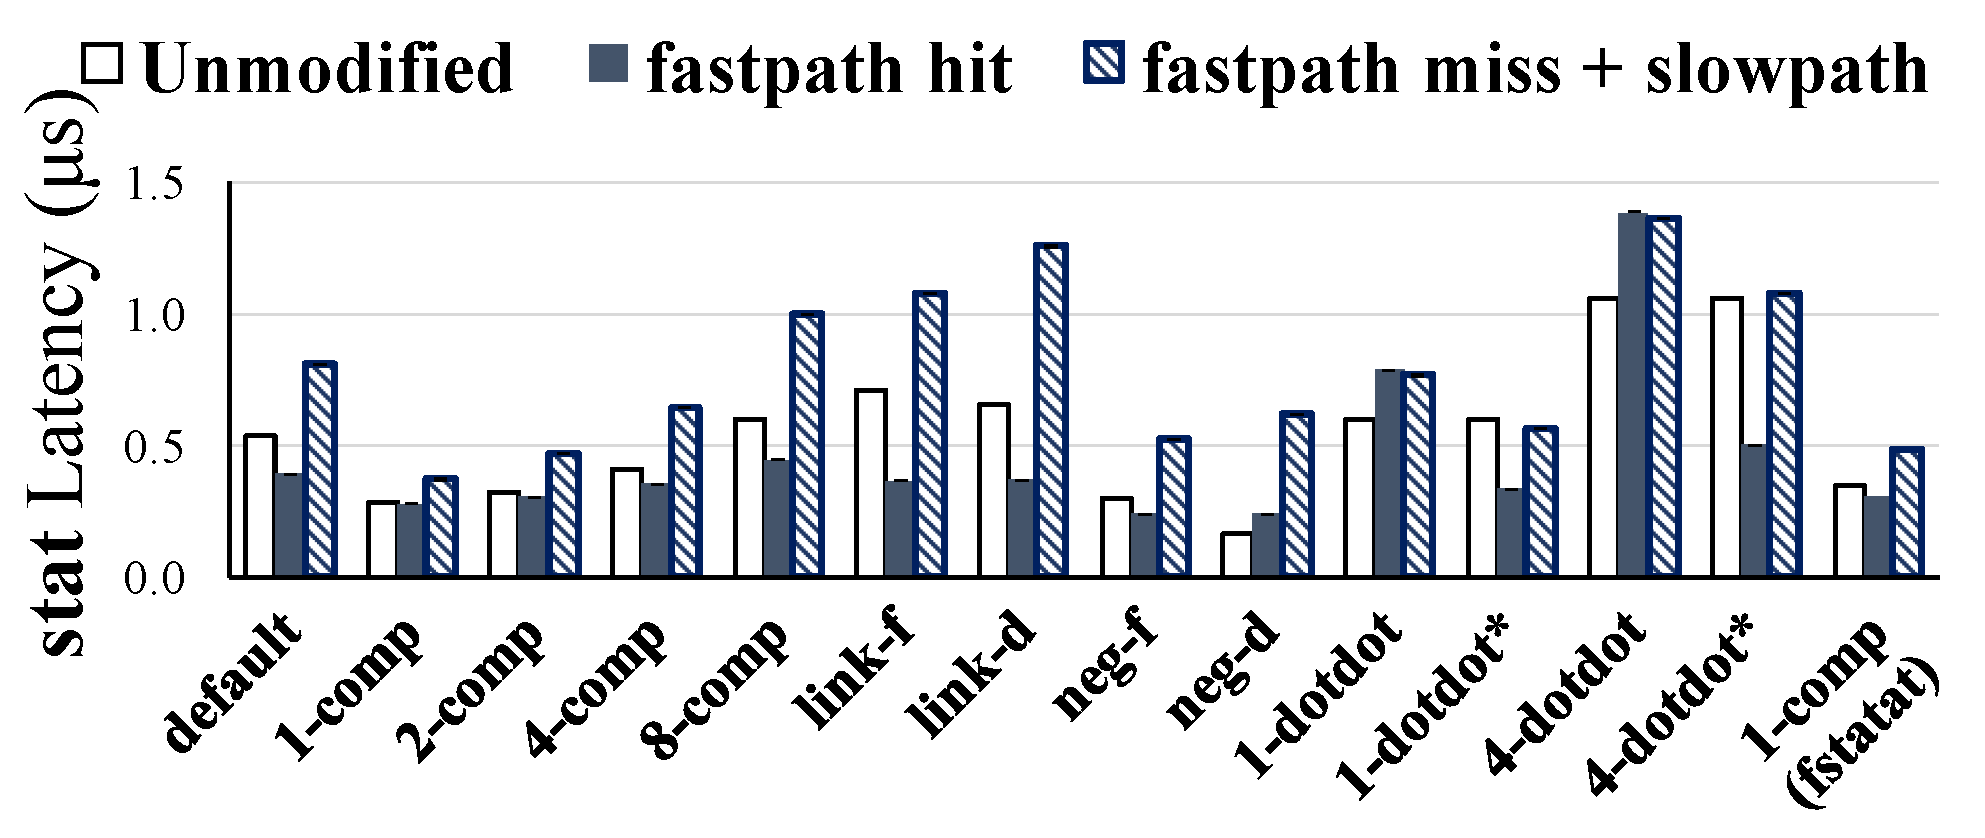
\includegraphics[width=3.6in]{dcache/plots/lm_stat.pdf} \\
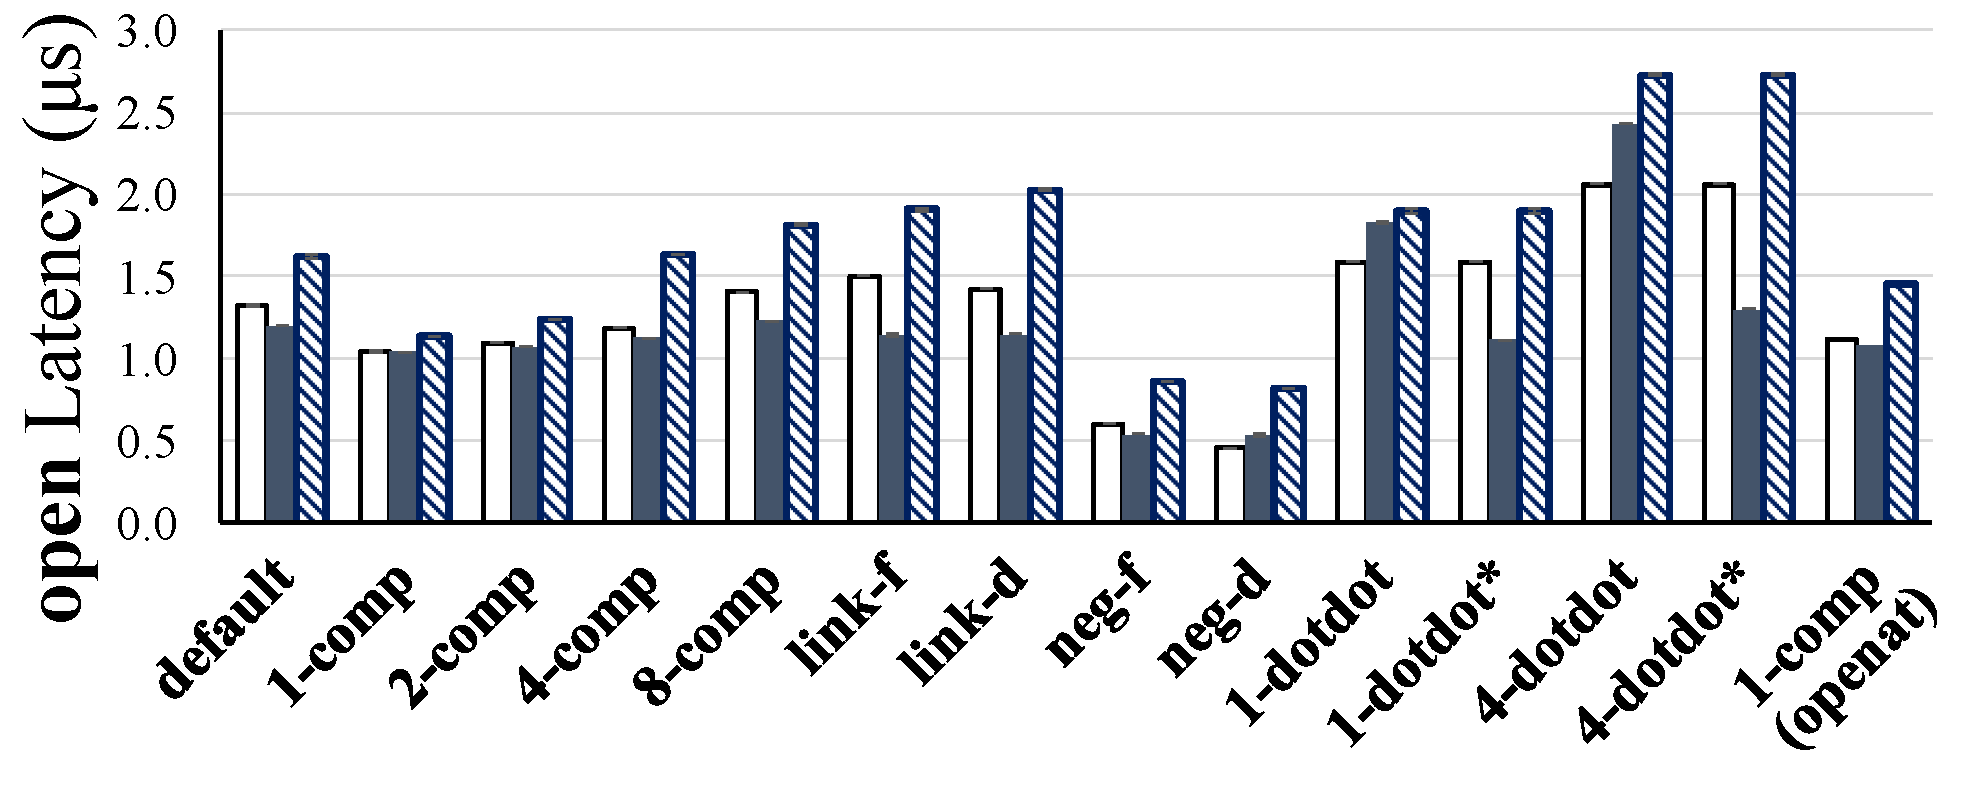
\includegraphics[width=3.6in]{dcache/plots/lm_open.pdf} \\
\end{minipage}
\begin{minipage}{2.6in}
\begin{tabular}{ll}
\multicolumn{2}{l}{({\bf * represents Plan 9's lexical parent semantics})} \\
\multicolumn{2}{l}{{\bf default:} \tt /usr/include/ ... /sys/types.h} \\
{{\bf 1-comp:} \tt FFF} &
{{\bf 2-comp:} \tt XXX/FFF} \\
\multicolumn{2}{l}{{\bf 4-comp:} \tt XXX/YYY/ZZZ/FFF} \\
\multicolumn{2}{l}{{\bf 8-comp:} \tt XXX/YYY/ZZZ/AAA/BBB/CCC/DDD/FFF} \\
\multicolumn{2}{l}{{\bf link-f:} \tt XXX/YYY/ZZZ/LLL -> FFF} \\
\multicolumn{2}{l}{{\bf link-d:} \tt LLL/YYY/ZZZ/FFF -> XXX/YYY/ZZZ/FFF} \\
\multicolumn{2}{l}{{\bf neg-f:} \tt XXX/YYY/ZZZ/NNN (NNN not found)} \\
\multicolumn{2}{l}{{\bf neg-d:} \tt NNN/XXX/YYY/FFF (NNN not found)} \\
\multicolumn{2}{l}{{\bf 1-dotdot:} \tt XXX/../FFF} \\
\multicolumn{2}{l}{{\bf 4-dotdot:} \tt XXX/YYY/../../AAA/BBB/../../FFF} \\
\end{tabular}
\end{minipage}
\caption[The optimized {\tt stat} and {\tt open} latency.]
{System call {\tt stat} and {\tt open} latency for micro-benchmark ({\tt lat\_syscall} in {\tt LMBench}), based on different path patterns. 
We include a synthetic evaluation of always missing on the fastpath and falling back to the slowpath,
and a comparison with Plan 9's lexical parent semantics, where appropriate.
Lower is better.}
\label{fig:dcache:stat-open}
\end{figure}

\paragraph{Micro-benchmarks.}
We use an extended LMBench 2.5 UNIX microbenchmark suite~\citep{McVoy:lmbench}
to evaluate latency of path lookup at the system call level.
%The {\tt lat\_syscall} test in {\tt LMBench} simply uses {\tt stat} or {\tt open} system calls repeatedly to access specific paths.
%We exercise the test with three different paths: root of a user home directory ({\tt /home/foo}), a important system header file with long path ({\tt /usr/lib/gcc/x86\_64-linux-gnu/4.6/stddef.h}) and a {\tt proc} file ({\tt /proc/sys/kernel/printk}).
%Generally {\tt lat\_syscall} demonstrates the best-case performance of directory cache lookup.
Figure~\ref{fig:dcache:stat-open} shows the latency to 
{\tt stat} and {\tt open} sample paths with various characteristics, 
including varying lengths, symbolic links, parent (dot dot) directories, 
and files that are not found.

The primary trend we observe is that, as paths have more components, 
the relative gain for our optimization increases.
For a single component file, {\tt stat} gains 3\% and open 
is equivalent to baseline Linux.
For longer paths, the gain increases up to 26\% and 12\%, respectively.
%For instance, a single component {\tt stat} only gains 1\%,
%whereas a four component {\tt sat} gains 27\%;
%the trends are similar for {\tt open}, except that one or two component paths perform slightly worse.


To evaluate the worst case, we include a set of bars, labeled ``fastpath miss + slowpath'', 
which exercise the fast path code, but the kernel is configured to always
miss in the PCC.  This simulates the full cost of executing the optimized fastpath unsuccessfully,
and then walking the O(n) slowpath in the cache.  This case 
does not miss all the way to the low-level file system.
The overhead typically ranges from 12--93\%,
%\fixmedp{update once we have spreadsheet}, 
except for path neg-d.
In the case of neg-d, the first component is missing, and a component-at-a-time walk
would stop sooner than a direct lookup. 
In general, the neg-d case would be mitigated by deep negative \dentries{}.
In practice, these overheads would only be observed 
for compulsory misses in the dcache, or by an application that exhibits
an extreme lack of locality.  

We next compare the costs of default Linux parent (``dot dot'') semantics 
to Plan 9's lexical semantics.  Enforcing 
Linux semantics for a path with parent references causes our optimizations
to perform roughly 31\% worse than unmodified Linux, as this requires an extra lookup 
per parent.
Lexical path semantics, on the other hand, allow our optimization to continue using a single
lookup, improving performance by 43--52\%.  Lexical path semantics
have an independent benefit, and could reduce the number of components
to walk in a lookup in unmodifed Linux.  
Although this difference is large, our test applications do not heavily use 
parent directory pointers, and are not sensitive to this difference.
%% Because this difference is so significant, and 
%% our applications generally do not follow symbolic links to parent directories 
%% (the main point at which the semantics yield different results),
%% we evaluate our application workloads using lexical path semantics.
%% \fixmedp{Does this actually matter?  Can we do it without lexical?}

Caching the resolution of a symbolic link improves 
performance for paths link-f and link-d by 44\% and 48\%, respectively.
This improvement is insensitive to where in the path the link occurs, 
as both link-f and link-d walk the same number of components (link-d maps ``LLL'' onto ``XXX'').

For files that do not exist (negative dentries), 
we see comparable improvements to paths that are present.  The one exception is
long paths that don't exist under a directory early in the path.
We believe this case is rare, as applications generally walk a directory tree top-down, rather than jumping
several levels into a non-existent directory.
In this situation (path neg-d), baseline Linux would stop processing the path faster
than our optimization can hash the entire path, even with caching deep negative dentries.
Nonetheless, deep negative dentries are an important optimization:
without them, stat of path neg-d would be 113\% worse 
and open would be 43\% worse than unmodified Linux, versus 38\% and 16\% slower with
deep negative dentries.

% Neg
%% stat Neg 2 .2444
%% open Neg 2 .5396

% NoNeg
%% stat Neg 2 .3732
%% open Neg 2 .6776


%% SOSP Space (and meh)
\begin{comment}
\begin{figure}
\scriptsize
\raggedleft
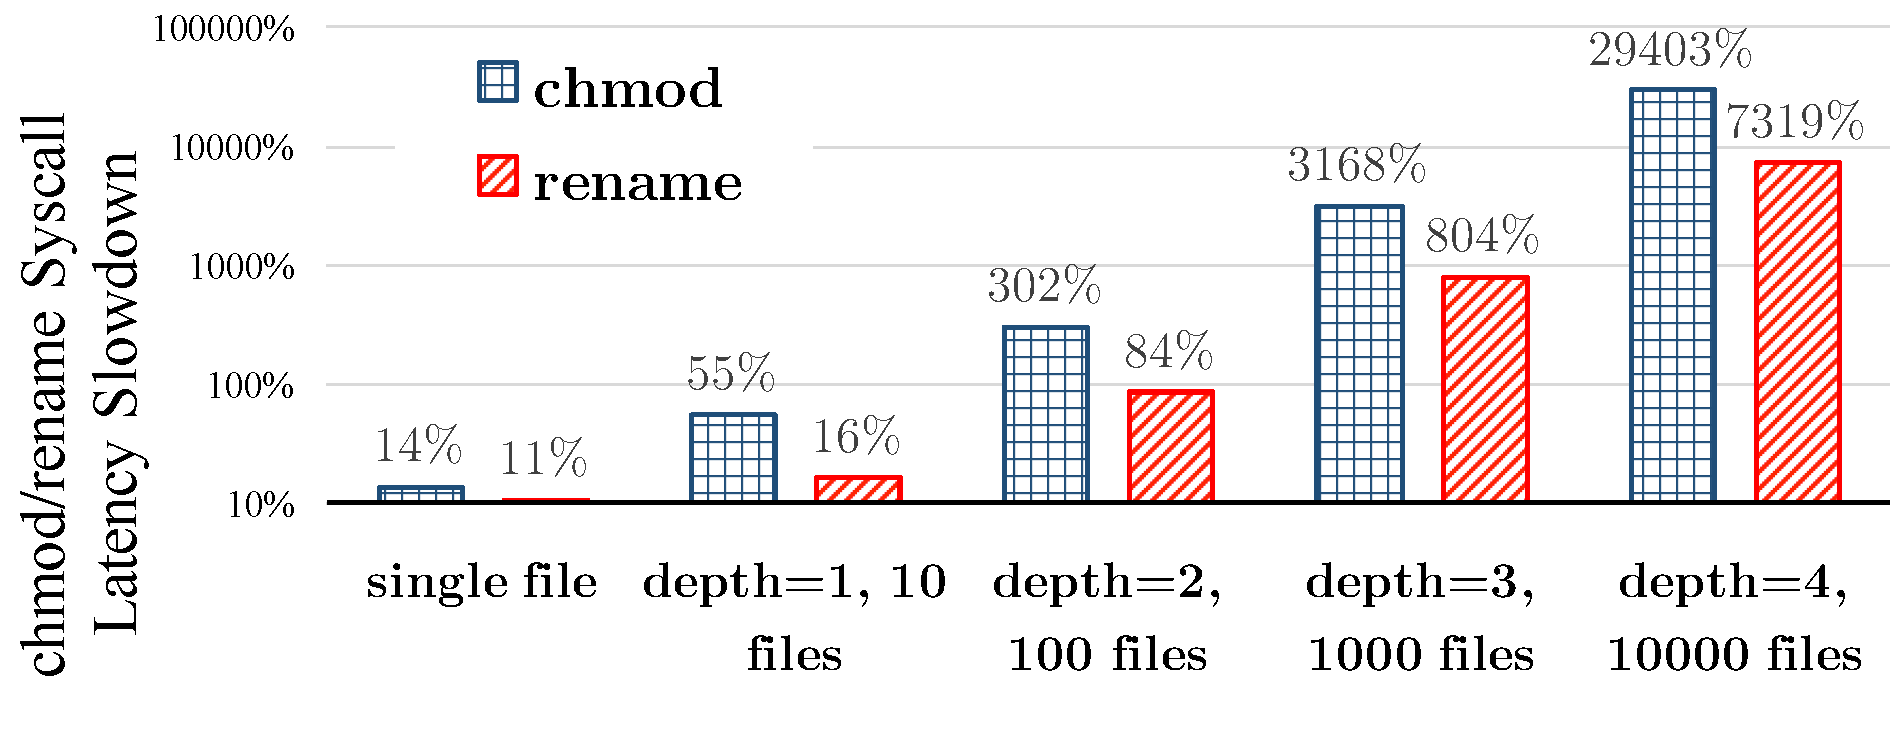
\includegraphics[width=0.9\linewidth]{dcache/plots/lm_rename-creat.pdf}
\vspace{-5pt}
\caption{Latency for micro-benchmarks that create and delete the same path in a loop. Lower is better.}
\label{fig:dcache:neg-dentry}
%\vspace{-10pt}
\end{figure}

%\paragraph{Renaming and Deletion.}

%We also show the benefits of better utilizing 
More aggressive use of 
negative dentries also benefits the case where a file is repeatedly created and deleted,
a pattern observed in applications such as text editors.
We measured this pattern with a micro-benchmark that renames and creates the same file, and a second
that opens and unlinks the same file.  These cases improved by roughly 6\% (Figure~\ref{fig:dcache:neg-dentry}).
%We also used the {\tt emacsclient} command line utility to save a few bytes to an empty file.
%Commensurate with the microbenchmark results, the improvement for this case was also 5\%.
Although editors tend to be I/O bound on the user, accelerating this pattern can reduce system load. 
\end{comment}


%% Longer paths show a more significant improvement, as the per-component costs in our
%% optimized kernel are much lower.
%% Even for single-component paths, our optimizations yield 6\% improvement for stat and 2\% for open;
%% the best-case improvements are over 58\%.

Linux also includes {\tt *at()} system call variants, which operate
under a working directory---typically using only a single component.
Commensurate with the results above, {\tt fstatat()}
benefits from our optimizations by 12\% 
for a single path component, and {\tt openat()} is 4\% faster than unmodified Linux.
Some applications use multiple-component names in conjunction with an {\tt *at} call;
in these cases, the benefit of our optimization is proportional to the path length.


\begin{figure}[t!]
\footnotesize
\centering
\begin{minipage}{5.3in}
\raggedleft
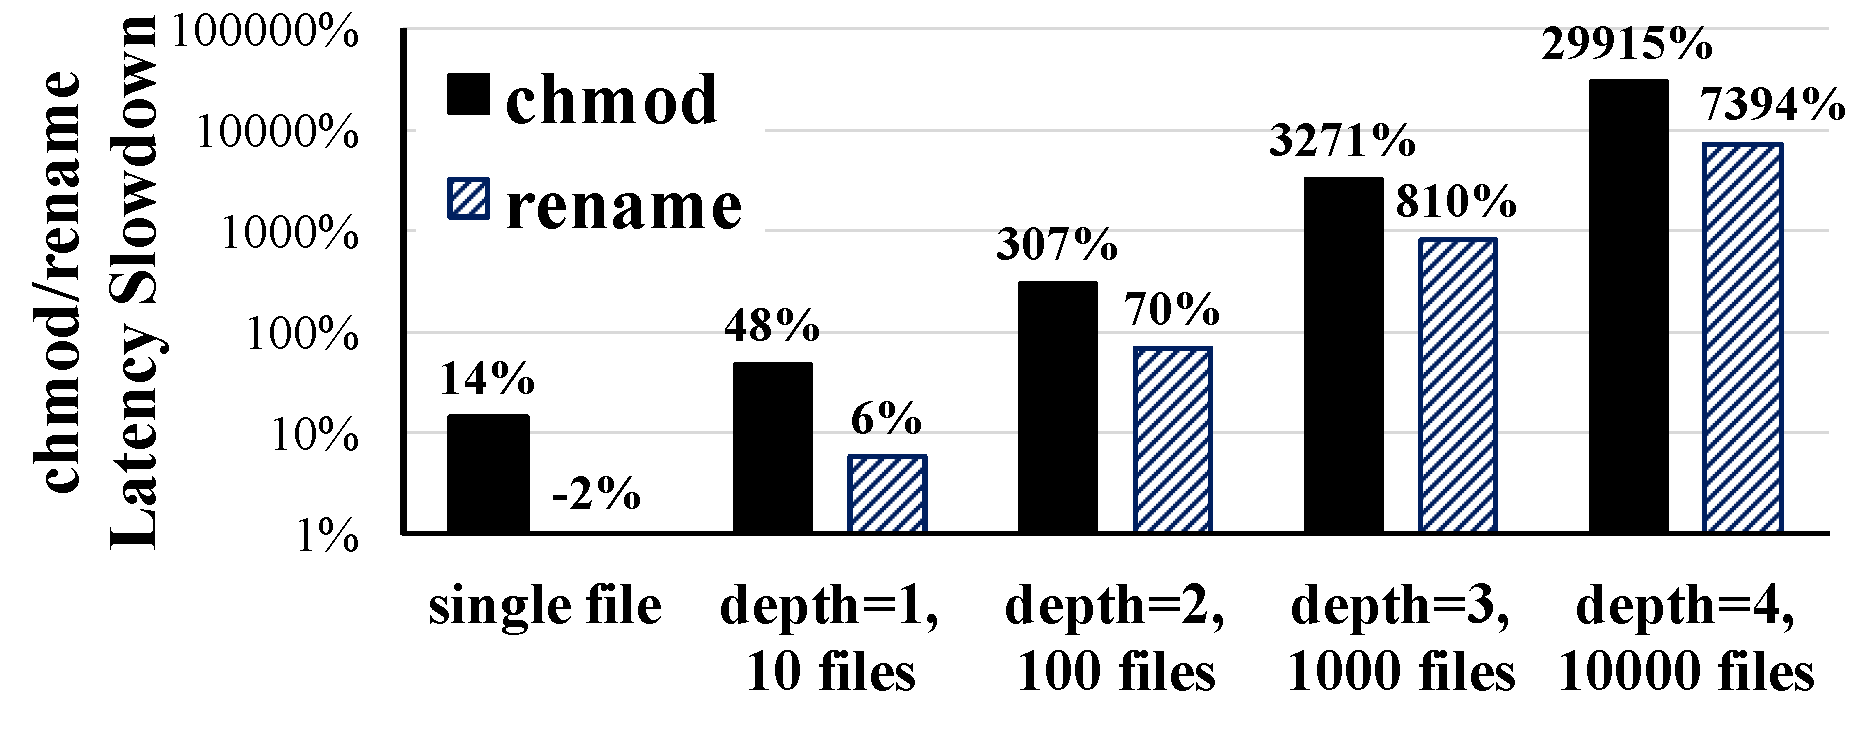
\includegraphics[width=5.4in]{dcache/plots/lm_chmod_rename.pdf}
{\setlength{\tabcolsep}{3pt}
\begin{tabular}{|l|R{.4in}R{.24in}|R{.4in}R{.24in}|R{.4in}R{.24in}|R{.4in}R{.24in}|R{.4in}R{.24in}|}
\hline
 & $\upmu$s & +/- & $\upmu$s & +/- & $\upmu$s & +/- & $\upmu$s & +/- & $\upmu$s & +/- \\
\hline
{\tt chmod}  & 1.86 & .00 & 1.60 & .00 & 4.37 & .00 & 36.38 & .01 & 323 & .02 \\
\hline
{\tt rename} & 3.73 & .00 & 4.68 & .00 & 7.51 & .00 & 40.14 & .01 & 330 & .05 \\
\hline
\end{tabular}}
\end{minipage}
\caption[Overhead of the {\tt chmod} and {\tt rename} latency in the optimized directory cache]
{{\tt chmod} and {\tt rename} latency in directories of various depths and sizes. Lower is better.}
\label{fig:dcache:chmod-rename}
\end{figure}

To evaluate the overhead of updating directory permissions and changing the directory structure,
we measure {\tt chmod} and {\tt rename} latency.
%We also wrote test cases for 
%creating and removing mount points,
%of different file system types such as {\tt ext4}, {\tt proc}, {\tt sysfs}, {\tt dev}
%and {\tt bind} mounts (logical aliases of other directories).
% {\tt lat\_perm} that makes {\tt chmod} system call on a directory,
%and then revalidates access permissions on every files in the directory by {\tt access} system call.
In our solution, the main factor influencing these overheads are the number of children
in the cache (directory children out-of-cache do not affect performance).
% are the depths and sizes (number of files) of the directory,
Figure~\ref{fig:dcache:chmod-rename} presents
performance of {\tt chmod} and {\tt rename}  on directories with different depths and directory sizes.
In general, the cost of a rename or chmod increases dramatically with the number of children,
whereas baseline Linux and ext4 make these constant-time operations.
Even with 10,000 children all in cache, the worst-case latency is around 330 $\mu$s.
As a point of reference, the Linux 3.19 source tree includes 51,562 files and directories.
Initial feedback from several Linux file system maintainers indicate that this trade would be acceptable
to improve lookup performance~\citep{linux-forum15}.

\begin{comment}
\begin{table}[t]
\scriptsize
\centering
\begin{tabular}{|l|rr|rrr|}
\hline
Types & \multicolumn{2}{c|}{Unmodified kernel} & \multicolumn{3}{c|}{Optimized kernel}  \\
& $\upmu$s & +/- & $\upmu$s & +/- & Overhead \\
\hline
{\tt ext4} & 0000.00 & .00 & 0000.00 & .00 & 00.0 \% \\
\hline
{\tt proc} & 0000.00 & .00 & 0000.00 & .00 & 00.0 \% \\
\hline
{\tt sysfs} & 0000.00 & .00 & 0000.00 & .00 & 00.0 \% \\
\hline
{\tt dev} & 0000.00 & .00 & 0000.00 & .00 & 00.0 \% \\
\hline
\end{tabular}
\caption{Latency of {\tt mount} / {\tt umount}, for creating and removing mount point based on file system types. Lower is better.}
\label{tab:dcache:mount}
\end{table}
\end{comment}

%We also evaluate the overhead of Table~\ref{table:lat_mount} shows the result of {\tt lat\_mount}, a {\tt LMBench} test case we extended, to measure latency of {\tt mount} and {\tt umount} system calls.

%\fixmedp{Why are make and make-j4 stats different?}

\begin{table*}[t]
\centering
\footnotesize
%\begin{tabular}{|l|R{0.12in}R{0.06in}|rrrr|rrr|rrr|rrr|}
\begin{tabular}{|l|R{0.5in}R{0.25in}|rrrr|rrr|}
\hline
Applications & \multicolumn{2}{c|}{Path Stats} & \multicolumn{4}{c|}{Unmodified kernel} 
%& \multicolumn{3}{c|}{Hit Optimization} & \multicolumn{3}{c|}{Miss Optimization} & \multicolumn{3}{c|}{All Optimizations} \\
& \multicolumn{3}{c|}{Optimized kernel} \\
& $l$ & \# & s & +/- & hit\% & neg\%  
%& s & +/- & Gain & s & +/- & Gain 
& s & +/- & Gain\\
\hline
{\tt find -name}
& 39 & 1
&   .055 & .000 &   100.0 &   .18
%&   0.045 & .000 & 18.5 \% 
%&   0.043 & .000 & 22.0 \%
&   .044 & .000 & 19.2 \% \\
\hline
\scalebox{.8}[1.0]{\tt tar xzf linux.tar.gz}
& 22 & 3
&   4.039 & .024 & 84.2 &   .06 
%&   4.037 & .011 &  .05 \%
%&   4.019 & .010 &  .05 \% 
&   4.038 & .010 &  .05 \% \\
\hline
\scalebox{.8}[1.0]{\tt rm -r linux src}
& 24 & 3
&   .607 & .008 &  100.0 &   .01 
%&   0.600 & .007 &  1.01 \%
%&   0.604 & .017 &   .45 \% 
&    .621 & .020 &  -2.32 \% \\
\hline
\scalebox{.8}[1.0]{\tt make linux src}
& 29 & 4
& 868.079 & .647 & 91.2 & 17.84 
%&     - &   - &     - \%
%& 868.3 & 1.1 & -0.02 \% 
& 868.726 & .892 & -.07 \% \\
\hline
\scalebox{.8}[1.0]{\tt make -j12 linux src}
& 29 & 4
& 102.958 & .597 & 92.9 & 20.03
%&     - &   - &     - \% 
%& 104.5 & 0.7 &  1.55 \%
& 103.308 & .288 & -.34 \% \\
\hline
{\tt du -s linux src}
& 10 & 1
&   .070 & .000 &  100.0 &   .01 
%&   0.058 & .000 &  17.08 \%
%&   0.057 & .000 &  18.69 \% 
&   .061 & .012 &  12.65 \% \\
\hline
{\tt updatedb -U usr}
&  3 & 1
&   .011 &  .000 & 99.9 &   .00 
%&   0.008 &  .000 & 29.41 \%
%&   0.008 &  .000 & 31.39 \% 
&   .008 &  .000 & 29.12 \% \\
\hline
\scalebox{.8}[1.0]{\tt git status linux src}
& 16 & 4
&   .176 &  .000 &  100.0 &  .05 
%&   0.167 &  .000 &  4.83 \%
%&   0.167 &  .000 &  4.75 \% 
&   .168 &  .000 &  4.26 \% \\
\hline
\scalebox{.8}[1.0]{\tt git diff linux src}
& 16 & 4
&   .066 &  .000 &  100.0 &  1.49
%&   0.063 &  .000 &  5.53 \%
%&   0.063 &  .000 &  5.55 \% 
&   .060 &  .000 &  9.89 \% \\
\hline
\end{tabular}
\caption[Directory cache optimization: application execution time (warm cache).]
{Execution time and path statistics of real-world applications bounded by directory cache lookup latency.  Warm cache case.  Hit rate and negative dentry rate are also included.  The average path length in bytes ($l$) and components (\#) are presented in the first two columns.  
%Optimizations for hits and misses are  presented separately, and then together.  
Lower is better.}
\label{tab:dcache:lookup-apps-warm}
\vspace{-10pt}

\end{table*}



%%% The cost of changing a directory's permissions ({\tt chmod}) is 12--16\%, depending on how many subdirectories are cached.
%%% We note that changing a file's permission incurs less than 2\% overhead.  We expect that permission changes to 
%%% high-level directories be very infrequent in practice---generally by an administrator; thus, a sub-second cost is still acceptable.
%%% The overhead added to a directory {\tt rename} is roughly 1\%, primarily because {\tt rename} is
%%% already an order of magnitude more expensive than other path-based operations, because of its atomicity requirements.

\paragraph{Space Overhead.}
Our prototype increases the size of a dentry from 192 bytes to 280 bytes.
Our design also introduces a per-credential PCC of size \PCCsize{}, 
and a second, global hash table (the DLHT),
which includes $2^{16}$ buckets.
Because Linux does not place any hard limits on dcache size, except extreme under memory pressure, 
it is hard to normalize execution time to account for the space cost.
%We expect sacrificing extra space for performance is a good trade-off for most systems, except perhaps embedded systems.
%We leave quantifying the value of entries
On a typical system, the dcache is tens to hundreds of MB; increasing this by 50\% is likely within an acceptable 
fraction of total system memory.
Alternatively, if one were to bound the total dcache size, this induces
a trade-off between faster hits and fewer hits.  
%We expect that the latency reductions afforded by our lookup optimizations make fewer entries 
%more valuable than more entries in many cases.  
%Alternatively, one could mix dentry sizes, allocating less space for infrequently accessed paths.
We leave exploration of these trade-offs for future work.

%% SOSP SPACE (and time); maybe for journal?
%\fixmedp{low-prio - F4 and F5 Evaluation with a memory budget, and microbenchmark with varying percentages of reuse, etc}

\begin{figure}[t!]
\footnotesize
\centering
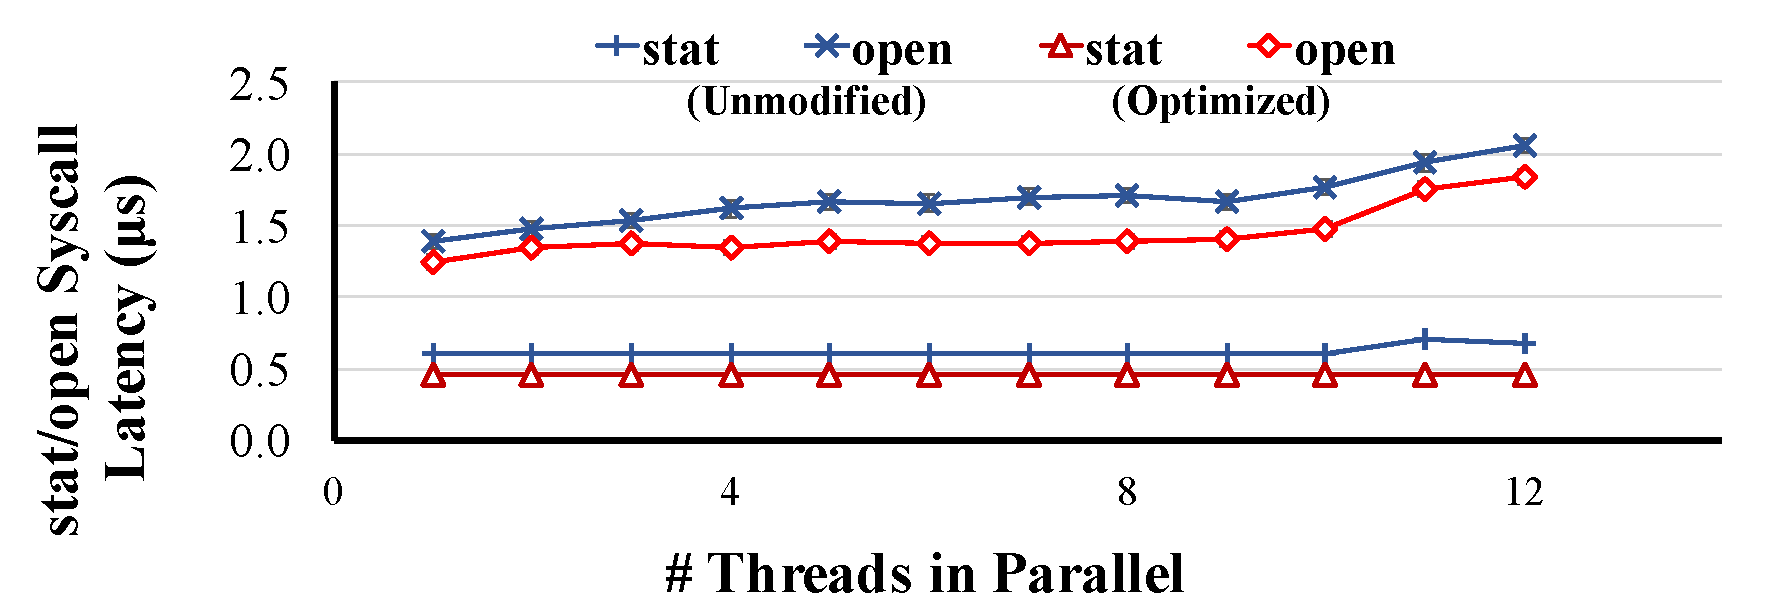
\includegraphics[width=5.5in]{dcache/plots/stat-open-scal.pdf}
\vspace{-5pt}
\caption[The optimized {\tt stat} and {\tt open} latency when called in parallel.]
{Latency of {\tt stat} and {\tt open} (of the same path) as more threads execute in parallel.  Lower is better.}
\label{fig:dcache:scalability}
%\vspace{-10pt}
\end{figure}



\paragraph{Scalability.}
Figure~\ref{fig:dcache:scalability} shows the latency of a {\tt stat/open} on the same path as more threads execute on the system.  
The read side of a lookup is already linearly scalable on Linux, and our optimizations do not disrupt this trend---only improve the latency.
The {\tt rename} system call introduces significant contention, and is less scalable in baseline Linux.
For instance, a single-file, single-core rename takes 13$\upmu$s 
on our test system running unmodified Linux; 
at 12 cores and different paths, the average latency jumps to 131$\upmu$s
for our optimized kernel, these numbers are 18 and 118$\upmu$s, respectively, indicating that 
our optimizations do not make this situation worse for renaming a file.
As measured in Figure~\ref{fig:dcache:chmod-rename},
our optimizations do add overhead to renaming a large directory, which would likely exacerbate this situation.
%\marginpar{\scriptsize \textcolor{blue}{Missing consistent data for opt kernel; have some data on a different machine}}

\subsection{Caching Directory Completeness}

\begin{figure}
\scriptsize
\centering
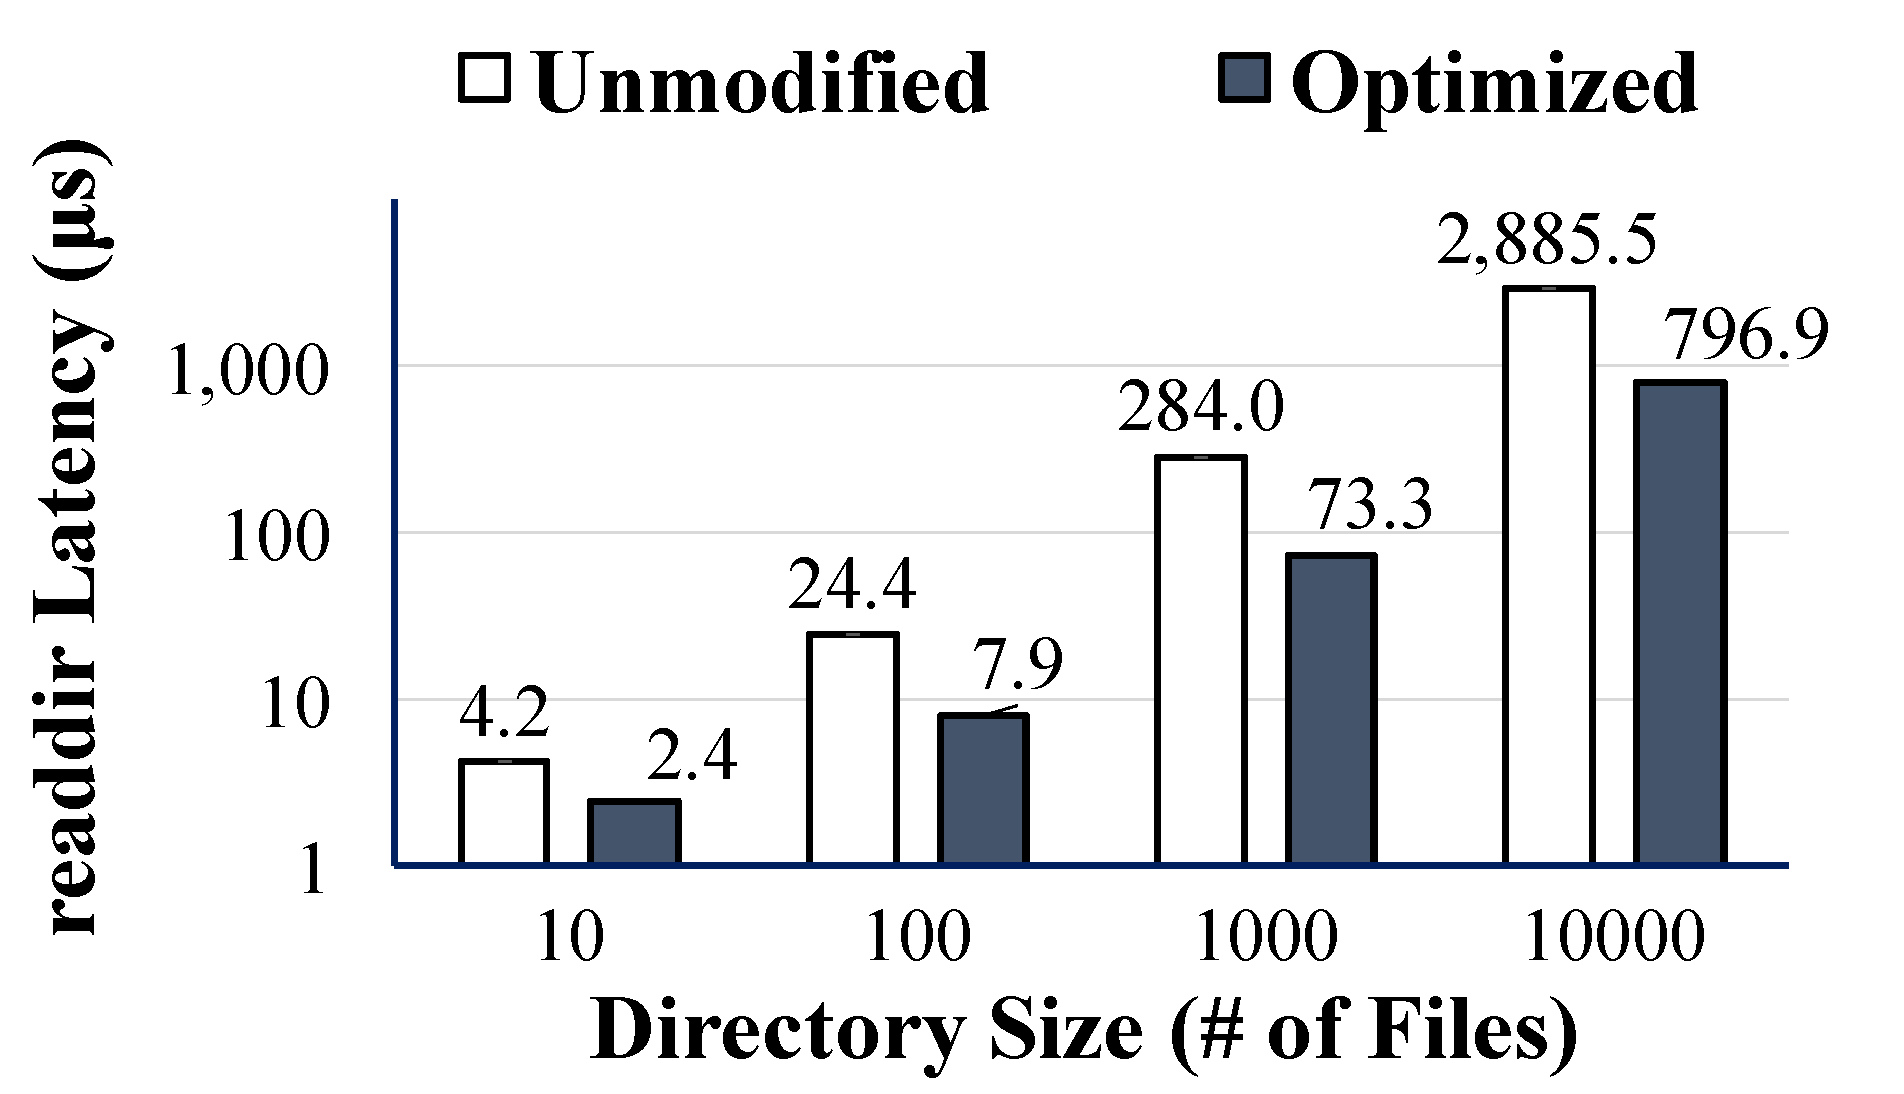
\includegraphics[width=3in]{dcache/plots/lm_readdir.pdf}
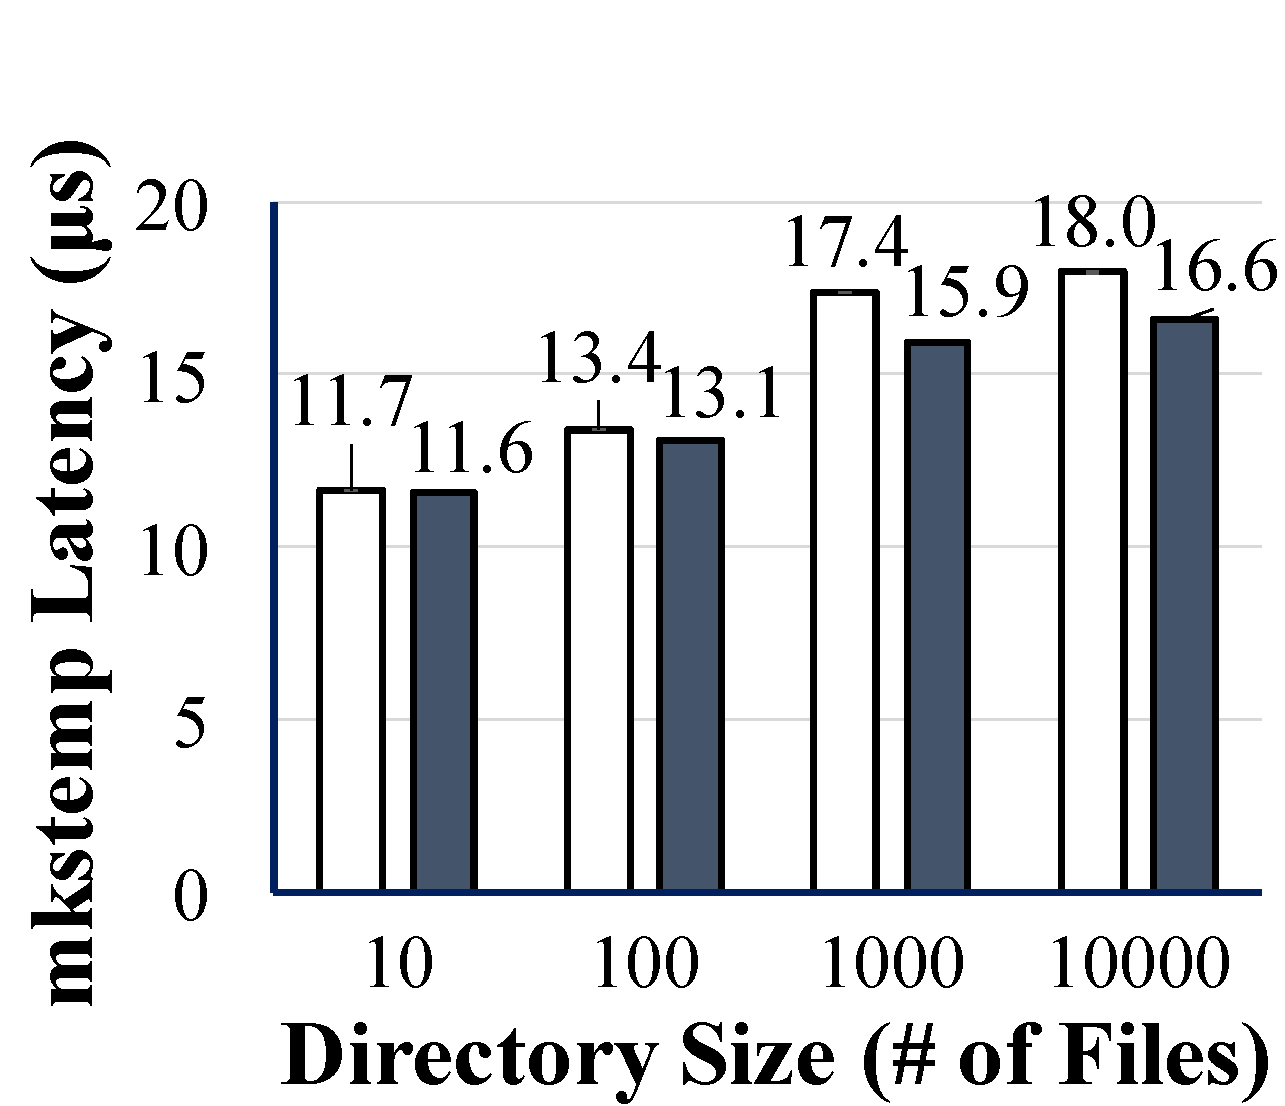
\includegraphics[width=3in]{dcache/plots/lm_mkstemp.pdf}
\caption[The optimized {\tt readdir} and {\tt mkstemp} latency.]
{Latency in logscale for {\tt readdir} function calls, and latency in microsecond for {\tt mkstemp} function calls, on directories with different sizes. Lower is better. }
\label{fig:dcache:readdir}
\end{figure}

%\paragraph{Micro-benchmarks.}
Figure~\ref{fig:dcache:readdir} shows the latency 
of a {\tt readdir} micro-benchmark with varying directory sizes.
%%% results of improving cache misses for listed directories.
%%% In both original and optimized kernel, the latency of directory listing, using {\tt getdents} or {\tt getdents64} system call,
%%% is relevant to the size (number of files) of the directories.
%%% We create a {\tt LMBench} test case {\tt lat\_readdir} to evaluate average time for listing 1000 directories, using {\tt getdents} system call.
%%% Each target directory in the test case is populated with given number of files before listing it.
The ability to cache {\tt readdir} results improves performance by 46--74\%.
%We omit cold cache data for brevity, which is an extremely noisy function of disk block placement, and shows no clear trend.
Caching helps more as directories get larger.
OpenSolaris comments indicate that this idea was only beneficial 
in UFS for directories with at least 1,024 entries~\footnote{see line 119 of {\tt fs/ufs/ufs\_dir.c} in OpenSolaris, latest version of frozen branch onnv-gate.}.
%there is a conventional wisdom that this is only useful for at least 1,024 entries and larger;
Our result indicates that there is benefit even for directories with as few as 10 children.

Figure~\ref{fig:dcache:readdir} also shows 
the latency of creating a secure, randomly-named file in directories of varying size.
We measure from 1--8\% improvement for the {\tt mkstemp} library.
Although most applications' execution times are not dominated by secure file creation,
it is a common task for many applications, and of low marginal cost.

%We measured cold cache numbers from this case, i.e., that are from a freshly rebooted system.
%as manually flushing the dcache through {\tt /proc} keeps the disk data cached.
%This data is extremely noisy, and, although our kernel reports a slowdown, both values are still within 
%experimental noise, despite multiple experiments.

%% SOSP Space (and meh)
\begin{comment}
\begin{figure}
\scriptsize
\raggedleft
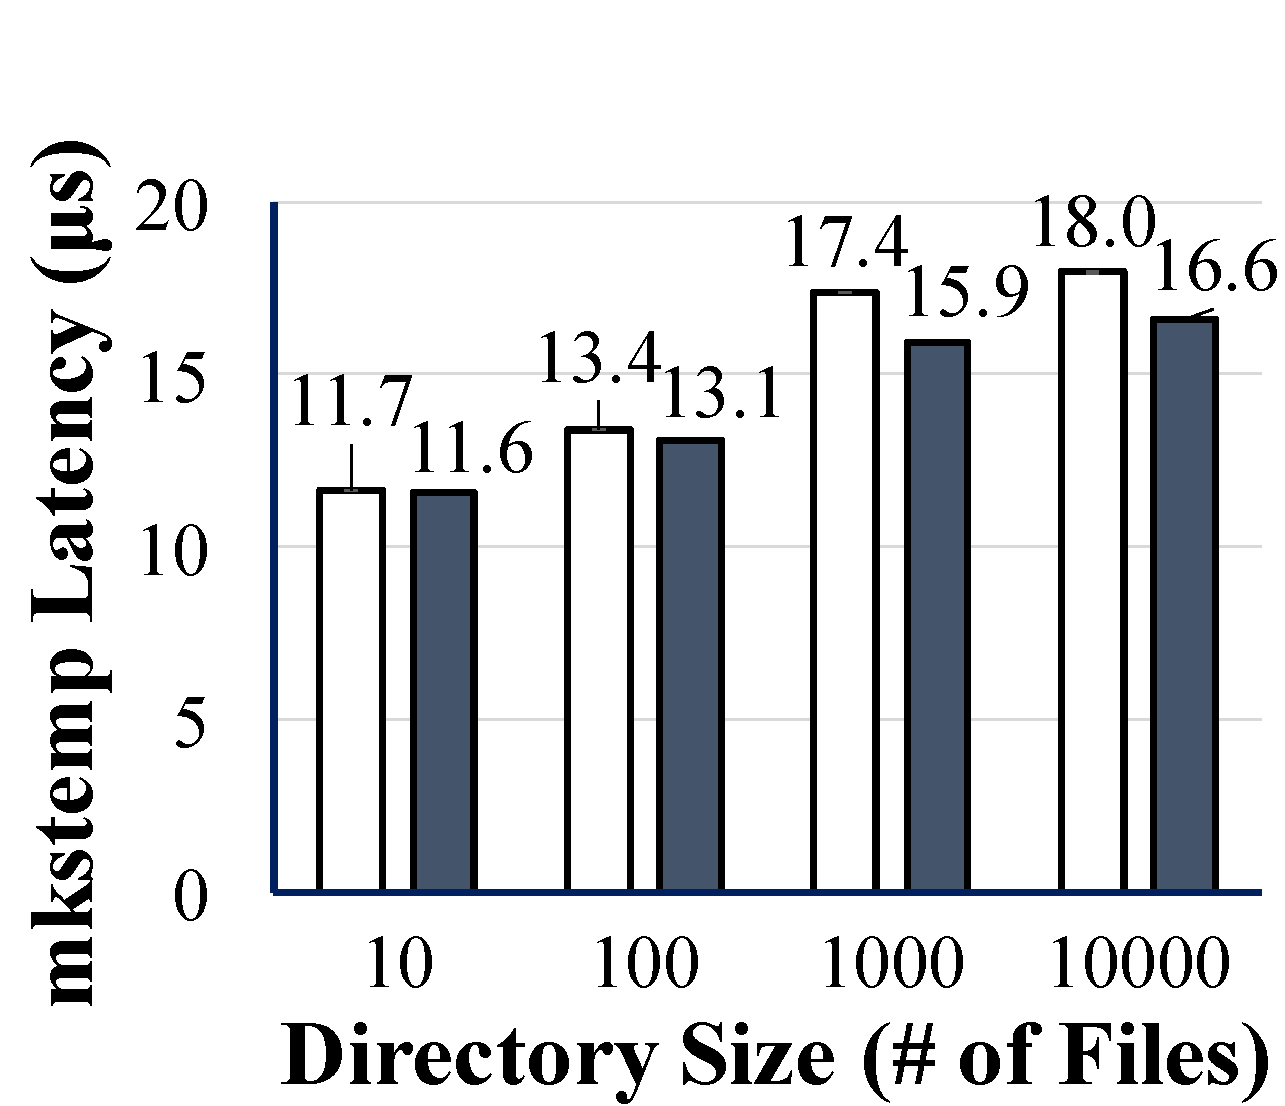
\includegraphics[width=0.9\linewidth]{dcache/plots/lm_mkstemp.pdf}
\caption{Latency of using {\tt mkstemp} to create unique file names in directories of different sizes. Lower is better.}
\label{fig:dcache:mktemp}
%\vspace{-10pt}
\end{figure}

\fixmedp{Mkstemp - what is going on with this data?  Need to answer D15}

\paragraph{File Creation in Completed Directories.}
We measure the latency of creating a secure, randomly-named file in directories of varying size.
We measure from 0--7.6\% improvement for the {\tt mkstemp} library, listed in Figure~\ref{fig:dcache:mktemp}. 
Although most applications' execution times are not dominated by secure file creation,
it is a common task for many applications, and of low marginal cost.

\end{comment}

\subsection{Applications}

\paragraph{Command-Line Applications.}
The improvement applications see from faster lookup is, of course, proportional 
to the fraction of runtime spent issuing path-based system calls as well as the amount of time
listing directories.
We measure the performance of a range of commonly-used applications.
In most cases, these applications benefit substantially from these optimizations;
%several commonly-used applications 
in the worst case, the performance harm is minimal.
%Gain for applications depends on whether they has significant ratio of metadata operations,
%and whether they access file systems with temporal locality.
%Based on these criterions, we choose applications
%that are excessively used in practice,
%to determine whether our optimization is truly beneficial for real-world use cases.
The applications we use for benchmarking include:
\begin{compactitem}
\item {\tt find}: search for a file name in the Linux source directory.
\item {\tt tar xzf}: decompress and unpack the Linux source.
\item {\tt rm -r}: remove the Linux source tree.
\item {\tt make} and {\tt make -j12}: compile the Linux kernel.
\item {\tt du -s}: Recursively list directory size in Linux source.
\item {\tt updatedb}: rebuild database of canonical paths for commonly searched file names in /usr from a clean {\tt debootstrap}.
\item {\tt git status} and {\tt git diff}: display status and unstaged changes in a cloned Linux kernel git repository.
\end{compactitem}
For each application we test, we evaluate the performance in both cases of 
a warm cache (Table~\ref{tab:dcache:lookup-apps-warm}) and a
a cold cache (Table~\ref{tab:dcache:lookup-apps}).
To warm the cache, we run the experiment once and drop the first run.
For the warm cache tests, we also provide statistics on the path characteristics of each application.
%% as well as evaluate the optimizations individually and together.

%Table~\ref{table:lookup-apps} shows the results of application performance.
%\fixmedp{Might be good to have a few more cases that change things, like a software install/remove?}

%\fixmedp{Stats for application benchmarks: cache hit/miss rate, non-existent path rate and effective cache occupancy }
%\fixmedp{I'd like to see Table 3 (warm) with each optimization individually, and then together}
%\marginpar{\scriptsize \textcolor{blue}{If time and space, add: cache hit/miss rate, non-existent path rate and effective cache occupancy}}

Perhaps unsurprisingly, metadata-intensive workloads benefit the most from our optimizations,
such as {\tt find} and {\tt update\-db}, as high 
as 29\% faster.  
Note that {\tt find}, {\tt update\-db}, and {\tt du} 
use the {\tt *at()} APIs exclusively, and all paths are single-component;
these gains are attributable 
to both improvements to lookup and 
directory completeness caching. % (see the split for miss vs. hit optimizations).

We note that the performance of directory-search workloads is sensitive to the size of PCC;
when we run {\tt updatedb} on a directory tree that is twice as large as the PCC, 
the gain drops from 29\% to 16.5\%.  This is because an increased fraction of the first
lookup in a newly-visited directory will have to take the slowpath.
Our prototype has a statically-set PCC size and 
we evaluate with a PCC sufficiently large to cache most of the relevant directories in 
the warm cache experiments.  We expect that a production system would dynamically resize the 
PCC up to a maximum working set; we leave investigating an appropriate policy to
decide when to grow the PCC versus evict entries for future work.

The application that is improved primarily by our hit optimization is {\tt git},
which shows a gain of 4--9.9\%. %, primarily attributable to the lookup optimizations.
%Even  
%a recursive remove, which modifies the directory tree one leaf at a time, was 2\% faster.
Cases that are dominated by other computations, such as a Linux compile, show minimal ($\le 2.3\%$ slowdown).
In the cold cache cases, all gains or losses are roughly within experimental noise, 
indicating that these optimizations are unlikely to do harm to applications
running on a cold system.
In general, these results affirm that common Linux applications will not be harmed by 
the trade-offs underlying our optimizations, and can benefit substantially.
%\fixmedp{Why are find, updatedb and du faster with *at calls?}
%\fixmedp{Why is git status not as good as git diff?}

%\subsection{Synchronization Cost in Directory Cache}

%\fixmetsai{skip this part for now.}

\begin{table}[t]
\footnotesize
\centering
\begin{tabular}{|l|rrrr|rrr|}
\hline
App & \multicolumn{4}{c|}{Unmodified kernel} & \multicolumn{3}{c|}{Optimized kernel} \\
& s & +/- & hit\% & neg\% & s & +/- & Gain \\
\hline
{\tt find}                         &    1.39 &  .01 &  38 &  1 &   1.35 &  .02 &  3.1 \% \\
\hline
\scalebox{.8}[1.0]{\tt tar}        &    4.00 &  .10 &  85 &  0 &   3.98 &  .04 &   .5 \% \\
\hline
\scalebox{.8}[1.0]{\tt rm -r}      &    1.81 &  .05 &  83 &  1 &   1.84 &  .06 & -1.4 \% \\
\hline
\scalebox{.8}[1.0]{\tt make }      &  885.33 &  .31 & 100 & 45 & 883.88 & 2.03 & .2 \% \\
\hline
\scalebox{.8}[1.0]{\tt make -j12 } &  114.51 &  .60 & 100 & 47 & 114.54 &  .89 & .2 \% \\
\hline
\scalebox{.8}[1.0]{\tt du -s }     &    1.49 &  .01 &   6 &  0 &   1.46 &  .02 & 2.3 \% \\
\hline
{\tt updatedb}                     &     .73 &  .01 &  34 &  0 &    .74 &  .01 & -2.1 \% \\
\hline
\scalebox{.8}[1.0]{\tt git status} &    4.13 &  .03 &  62 &  2 &   4.11 &  .03 &  .7 \% \\
\hline
\scalebox{.8}[1.0]{\tt git diff}   &     .84 &  .01 &  61 &  0 &    .86 & .01 & -14.0 \% \\
\hline
\end{tabular}
\caption[The optimized application execution time (in cold cache).]
{Execution time, hit rate, and negative \dentry{} rate for real-world applications bounded by directory cache lookup latency with a cold cache. Lower is better.}
%\vspace{-10pt}
\label{tab:dcache:lookup-apps}
\end{table}



\begin{comment}
The impact of hit and miss optimizations are not strictly additive.
We believe there are two reasons for this.  First, additional bookkeeping 
for more optimizations can cause the dentry to span more cache lines, lowering 
locality.  We attribute this to cases such as {\tt git diff}, where adding directory
completeness lowers performance relative to the hit optimizations alone.
In other cases, such as {\tt du}, the hit optimizations alone are a wash \fixmedp{if new numbers justify this}, but
the two combine to more than the sum of the parts.
We attribute this effect to the preceeding {\tt readdir} is populating the cache,
improving the hit rate for the fastpath lookup. 
\fixmedp{Can we get stats  to confirm this suspicion?}
\end{comment}

Table~\ref{tab:dcache:lookup-apps-warm} also indicates statistics about these workloads
on unmodified Linux.  
%First, we measure the average path length (in characters),
%and components.  
In general, each path component tends to be roughly 8 characters, 
and *at-based application generally lookup single-component paths, 
%looked-up paths have one component (for *at-based applications), 
whereas other applications typically walk 3--4 components.  
Our statistics also indicate that, with a warm cache, these applications 
should see 84--100\% hit rate in the cache, so optimizing the hit path is essential to performance.
Finally, make is the only application with a significant fraction of 
negative \dentries{} (roughly 20\%),
which is to be expected, since it is creating new binary files.

%\fixmedp{Tput for Dovecot and apache}

\paragraph{Server Applications.}
An example of software that frequently uses {\tt readdir} is an
IMAP mail server using the MailDir storage format.
%will stores every mail in the mailbox as a file inside a directory, with file name formatted as a combination of timestamp, identifier and flags.
We exercise the Dovecot IMAP server by creating 10 mailboxes for a client.
We use a client script to randomly select messages in different mailboxes and mark them as read, flagged, or unflagged.
Internally, marking a mail causes a file to be renamed, and the directory to be re-read.
To eliminate network latency, we run network tests on the localhost; 
in a practical deployment, network latency may mask these improvements to the client, but the load of the server will still be reduced.

%will scan the directories of users' mailboxes constantly in order to track the status of all mails in consistent state.
%For evaluation, we create a Dovecot server with 10 mailboxes.
%In each mailbox, we store certain number of mails and use a client-side script written in Python (using {\tt ImapLib} library)
%to randomly mark or unmark 1000 mails with a specific flag.  
%After every time a client has marked or unmark a mail, the mail server will rename the file and rescan the whole directory for a updated list of mails. 


\begin{figure}
\scriptsize
%\raggedright
\centering
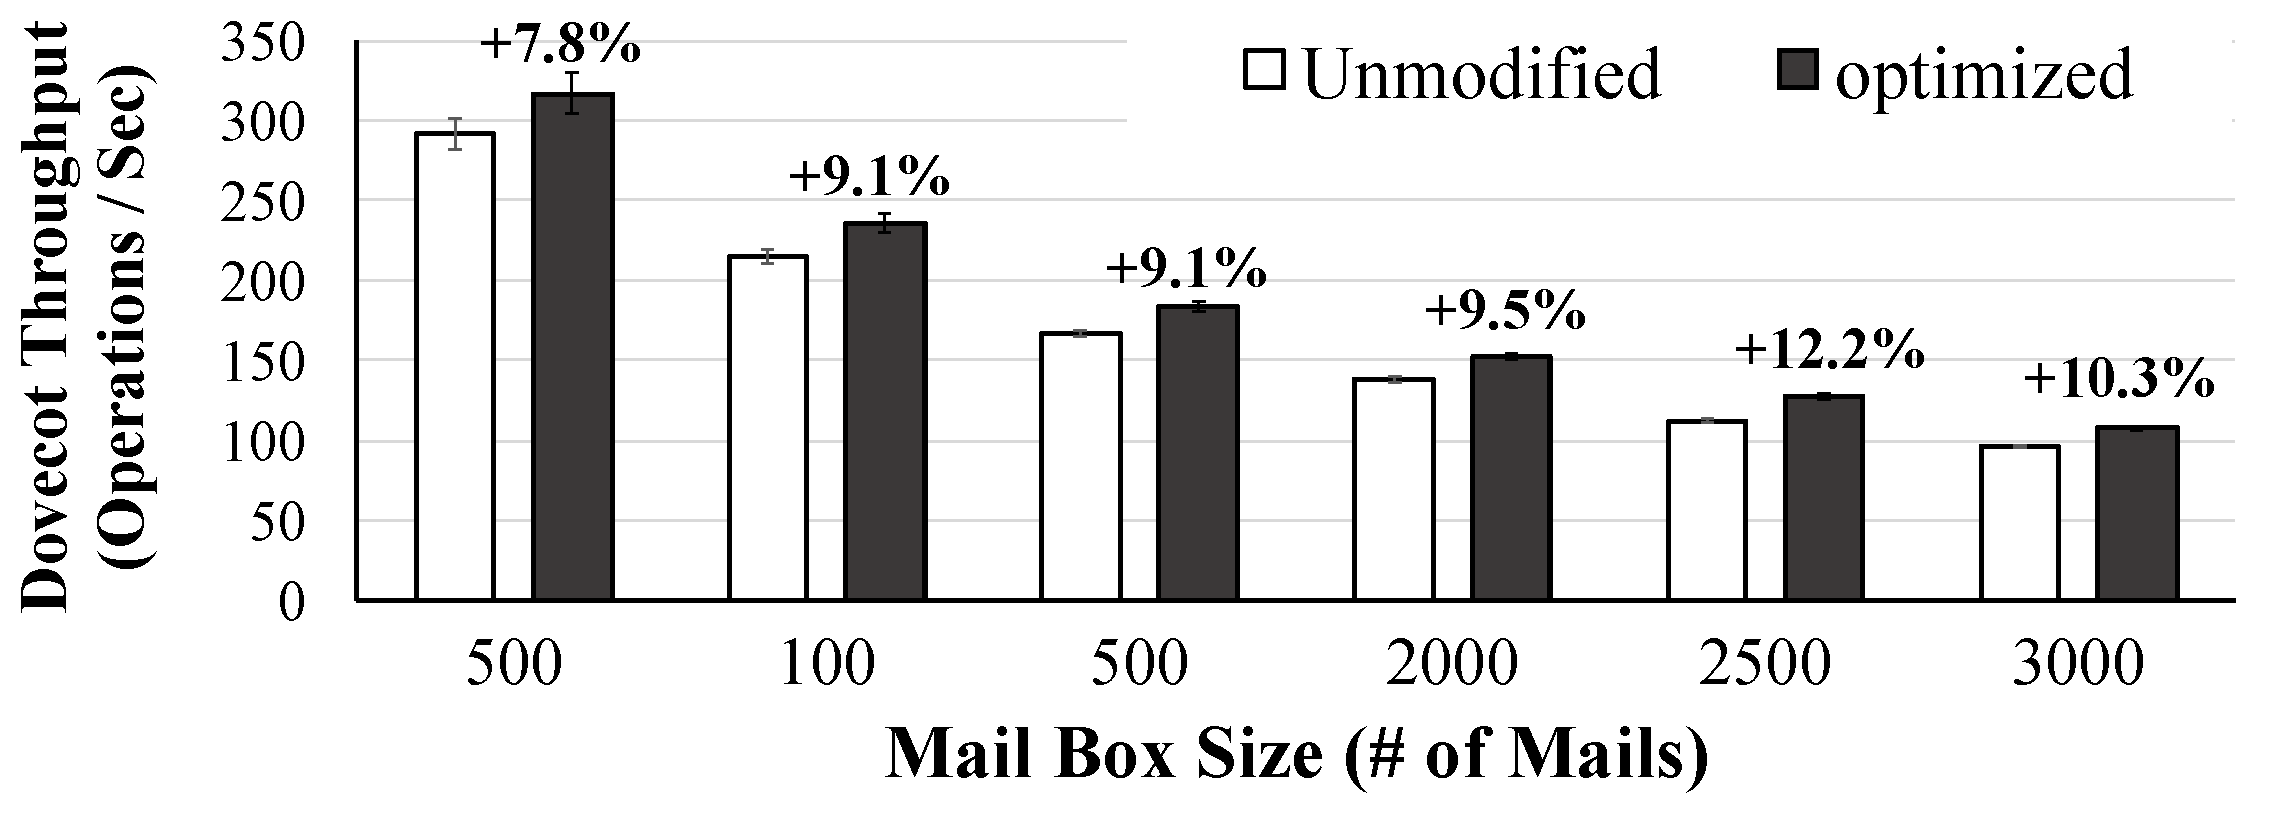
\includegraphics[width=5in]{dcache/plots/dovecot.pdf}
\vspace{-5pt}
\caption[Directory cache optimization: the Dovecot IMAP server throughput.]
{Throughput for marking and unmarking mail on the Dovecot IMAP server. Higher is better. }
% In the optimized kernel, throughputs of all workloads are improved by 5--11\%. }
\label{fig:dcache:dovecot}
\end{figure}

\begin{table}[t]
\footnotesize
\centering
\begin{tabular}{|c|rr|rrr|}
\hline
\# of files & \multicolumn{2}{c|}{Unmodified kernel} & \multicolumn{3}{c|}{Optimized kernel} \\
& Req/s & +/- & Req/s & +/- & Gain\\
\hline
    10 &     27,638.23 & 43.31 & 31,491.98 & 55.24 & 12.24 \% \\
\hline
$10^2$ &      7,423.86 & 11.81 &  7,934.07 & 12.76 &  6.43 \% \\
\hline
$10^3$ &      1,017.02 &  0.58 &  1,081.02 &  0.38 &  5.92 \% \\
\hline
$10^4$ &         99.03 &  0.11 &    110.14 &  0.10 & 10.09 \% \\
\hline
\end{tabular}
\caption[The optimized Apache server throughput.]
{Throughput of downloading generated directory listing pages from an {\tt Apache} server. Higher is better.}
\label{tab:dcache:apache}
\end{table}

Figure~\ref{fig:dcache:dovecot} shows the throughput for the 
Dovecot mail server on both kernels; improvements range from 7.8--12.2\%.
Commensurate with the {\tt readdir} microbenchmark, larger directories 
generally see larger improvement, plateauing at a 10\% gain.
%perform better, but even small mailbox sizes benefit from the optimization.
We similarly exercise the Apache web server's ability to generate a file listing using the Apache benchmark (Table~\ref{tab:dcache:apache}).
These pages are not cached by Apache, but generated dynamically for each request.
This workload also demonstrates improvements in throughput from 6--12\%.
%Similar to previous results, the throughput improvement is linear in the
%size of the directory (up to 9.48\%), although small (10 file) directories lose 6\%.
%\fixmedp{Why; this is not the case in our microbenchmark.}
%For small directories (10 files), our system reduces throughput by 6\%;
%for larger directoires, the throughput increases 
%Similar to the previous results, the average file listing is 2--10\% faster. 
Overall, these results show that the readdir caching strategy can reduce server load
or improve server throughput for directory-bound workloads.
%and improve client response time.

\begin{comment}
\begin{table}[t]
\scriptsize
\centering
\begin{tabular}{|l|rr|rrr|}
\hline
Target & \multicolumn{2}{c|}{Unmodified kernel} & \multicolumn{3}{c|}{Optimized kernel} \\
& s & +/- & s & +/- & Gain\\
\hline

\hline
{\tt logrotate} & 000.00 & .00 & 000.00 & 0.00 & 00.0 \% \\
\hline
\end{tabular}
\caption{Latency of applications that constantly {\tt rename/creat} or {\tt unlink/creat} files or directories. Lower is better.}
\label{tab:dcache:neg-dentry-apps}
\end{table}
\end{comment}

%%% Avoiding cache misses for file creation after renaming or deletion is more likely an optimization beneficial system-wide.
%%% Only very few applications we found have the same scenario of repeatedly renaming/deleting files and recreating them.
%%% Some of the applications are text editors such as {\tt vim} or {\tt emac}.
%%% When a user is editing a file, the editors will create a copy of the file as temporal snapshot, and rename the file to the actual name when user saves the edit.
%%% The scenario of renaming and recreating files happens when user constantly saves and continues editing files.
%%% Another use case is system scripts such as {\tt logrotate} will use renaming as an atomic way of updating files,
%%% and the script will constantly rename existent files or directories as unique new names and recreate them.
%%% Table~\ref{table:neg-dentry-apps} shows the results of the applications we choose, including {\tt emac} and {\tt logrotate}.  

%%% \fixmetsai{Observation here}

%\paragraph{Deep Negative \dentries{}.} 
%%%%%\fixmetsai{skip this part for now.}

\subsection{Code Changes}

In order estimate the difficulty of adoption, Table~\ref{tab:dcache:loc} lists the lines of code changed in our Linux prototype.
The vast majority of the changes required (about 1,000 LoC)
are hooks localized to the dcache itself ({\tt dcache.c} and {\tt namei.c});
most of these optimizations are in a separate set of files totaling about 2,400 LoC.
Also, the low-level file systems we tested did not require {\em any} changes to use our modified directory caches.
%TSAI: no longer needed, we just don't support them.
%although some file systems that use a custom hash function would require small changes.
The main impact on other subsystems was actually to the LSMs, which required some changes
to manage PCCs correctly. % CIDs correctly (4--13 LoC out of 4--16 kLoC).
%A few other changes were scattered throughout core kernel and VFS files, primarily to manage CIDs.
Thus, the burden of adoption for other kernel subsystems is very minor.

\begin{table}[t]
\footnotesize
\centering
%\subfloat[VFS layer]{
\begin{tabular}{p{3in}rrr}
Source files & \multicolumn{1}{c}{Original (LoC)} & \multicolumn{2}{c}{Patched/Added (LoC)} \\
\hline
%unifdef -DCONFIG_OPTIMIZE_DCACHE -U CONFIG_OPTIMIZE_DCACHE_CHECK_FULLPATH -DCONFIG_OPTIMIZE_READDIR -UCONFIG_OPTIMIZE_DCACHE_DEBUG -UCONFIG_OPTIMIZE_DCACHE_LOOKUP_NOBARRIER -UCONFIG_OPTIMIZE_DCACHE_REANAME_COPY DDENTRY_SIGNATURE_BITS=192 -DCONFIG_OPTIMIZE_DCACHE_RENAME_NEGATIVE -DCONFIG_OPTIMIZE_DCACHE_RENAME_NEGATIVE_CREATE -DCONFIG_OPTIMIZE_DCACHE_SIGNATURE_MHASH -DCONFIG_OPTIMIZE_DCACHE_PERM_CACHE_CID UCONFIG_DENTRY_LOOKUP_TIME -UCONFIG_PATH_LOOKUP_TIME -UCONFIG_DENTRY_ALLOCATE_TIME -UCONFIG_INODE_LOOKUP_TIME -DCONFIG_OPTIMIZE_READDIR_SKIP_LOOKUP  -UCONFIG_OPTIMIZE_DCACHE_SCAN_BACKWARD -UCONFIG_PATH_LOOKUP_BREAKPOINT -UCONFIG_OPTIMIZE_DCACHE_DUMMY  -DCONFIG_DCACHE_WORD_ACCESS -UCONFIG_OPTIMIZE_DCACHE_RENAME_COPY -UCONFIG_OPTIMIZE_DCACHE_STATISTICS -DCONFIG_MHASH_192 -UCONFIG_MHASH_128 -U CONFIG_OPTIMIZE_DCACHE_PROFILE -UCONFIG_OPTIMIZE_DCACHE_SIGNATURE_SIMPLE -UCONFIG_OPTIMIZE_DCACHE_SIGNATURE_JELKINS_OLD -UCONFIG_OPTIMIZE_DCACHE_SIGNATURE_JELKINS_LOOKUP3 -UCONFIG_OPTIMIZE_DCACHE_SIGNATURE_JELKINS_SPOOKY -UCONFIG_OPTIMIZE_DCACHE_SYMLINK_LOOKUP dcache.c > dcache-clean.c
% sloccount fs/dcache-clean.c
% just do make -f Makefile-cloc in the repo.
New source files \& headers  & & 2,358 & \\
\hline
{\tt fs/namei.c}   & 3,048 & 425 & 13.9 \% \\
\hline
{\tt fs/dcache.c}  & 1,997 & 142 &  7.1 \% \\
\hline
% fs/libfs.c fs/namespace.c fs/open.c fs/readdir.c
Other VFS sources  & 3,859 &  98 &  2.5 \% \\
\hline
% fs/internal.h fs/mount.h include/linux/dcache.h include/linux/fs.h include/linux/namei.h
Other VFS headers  & 2,431 & 218 &  9.0 \% \\
\hline
% include/linux/cred.h kernel/cred.c kernel/nsproxy.c security/apparmor security/selinux
Security Modules (SELinux, etc)   & 20,479 & 76 & 0.0 \% \\
\hline
\end{tabular}
\caption[lines-of-code changed in Linux for directory cache optimization]
{{\em Lines-of-code} (LoC) changed in Linux, as measured by {\tt sloccount}~\citep{sloccount}.}
\label{tab:dcache:loc}
%\vspace{-10pt}
\end{table}

%% difficulty of porting our code to a new Linux kernel, or supporting file system drivers implemented by third-parties.
%% To evaluate portability, we must measure two factors in our solutions: the first is {\em Line-of-code} (LoC) of our patch to the VFS layer in Linux kernels.
%% If the directory cache design in VFS layer is not significantly changed, our patch should be able to apply on new Linux kernels with no pain.
%% Otherwise, our solution may need to be partially reimplemented, based on new interfaces or assumption of kernel codes.
%% The second factor is {\em Line-of-code} of our changes in the code of individual file system drivers.
%% Our solution maintains minimal effort possible to fix file system drivers for making them compatible to the optimized directory cache.
%% The statistic of our solution is show in table~\ref{table:portability}.

\begin{comment}
\subsection{Compatibility}

Demonstrating bug-for-bug compatibility with any large body of software is 
always a challenge, and indicators are noisy.
As a step in this direction, we ran the file system regression test script from the Linux Test Project~\citep{linux-test}
and verified that they pass on our system.
We wrote additional tests that checked that permission handling behaved the same way on AppArmor and SELinux.
This gives us confidence that our prototype's path handling behavior will be transparent to applications.

\end{comment}

\begin{comment}
\subsection{Discussion and Future Work}

%\fixmedp{Chia-Che, please review this section.  Any of this to hold back (as in we might want to actually do this?}
If one were willing to sacrifice complete backward compatibility to maximize lookup performance,
the primary opportunity for improvement may actually be in designing a simpler 
{\em interface} for path-based calls.
As the evaluation above shows, there are several Linux/POSIX features
that are unduly expensive to support in this design.
For instance, implementing Plan 9-style lexical path semantics
can significantly improve look up for paths with a ``dot dot''.
Similarly, working directory semantics require
a slowpath traversal.
Arguably, these are points where a particular implementation choice
has ``leaked'' into the interface specification,
and these idiosyncracies constrain the choice of supporting data structure.
We recommend an interface that is as simple and stateless as possible; 
this recommendation is in line with other recommendations for scalability~\citep{clements13scalable}.


\fixmedp{Maybe vague this up?}
A contribution of this work is separating permission checking from finding 
a \dentry{} in the cache.  
In our design, we cache the results of prefix checks,
in part because of the diversity of policies
implemented in LSMs.
We also observe that directories with different permissions than their parents are relatively rare,
and this information is scattered across the file system in inode mode bits and extended attributes.
A directory cache with 
a higher-level, compact representation of the system's access control policies
might be able to replace prefix caching with efficient, inline policy evaluation.

\fixmedp{Maybe drop this?}
The Linux dcache is not completely RCU-compliant because a rename can 
move a dentry from one parent to another.  Even in unmodified Linux, this introduces 
the need for even more elaborate synchronization, such as a sequence lock and a retry loop
for concurrent lookup and rename of the same path.
This complexity could be reduced for the common case (lookup)
by making the cache completely RCU-compliant---i.e., 
copying or invalidating dentries under a renamed directory, rather than moving the parent with a pointer swing.



%% Total: 524288
%% bucket size 0: 305351 - 58%
%% bucket size 1: 177571 - 33.8%
%% bucket size 2: 36384 - 7%
%% 3+ <1%
%% bucket size 3: 4470 
%% bucket size 4: 460
%% bucket size 5: 41
%% bucket size 6: 5
%% bucket size 7: 2
%% bucket size 8: 2
%% bucket size 9: 1
%% bucket size 10: 1


Linux statically selects the number of buckets in the hash table (262,144 by default).
If this number is not selected well, or the demand changes over time,
space will be wasted or bucket chains will get longer, harming lookup performance.
On our test systems, 58\% of buckets were empty, 34\% had one item,
7\% had 2 items, and 1\% had 3--10 \dentries{},
indicating an opportunity to improve lookup time and space usage.
%\fixmedp{As an aside, what is the average and variance?  This seems like Linux's hash function is crappy and not getting an even distribution.}
A number of high-performance hash tables have been developed in recent years that
impose a constant bound on the search time as well as on wasted space~\citep{cuckoo04,li14cuckoo,triplett11hash,herlihy08hopscotch}.
%Based on our data,  we expect that a better hash table algorithm could also improve lookup time, in baseline Linux or our design.

\end{comment}